\documentclass[10pt]{article}

\usepackage[T1]{fontenc}
\usepackage[left=2cm, right=2cm, top=2cm, bottom=2cm, paperheight=31cm]{geometry}
\usepackage[skins]{tcolorbox}
\usepackage{hyperref, fancyhdr, lastpage, tocloft, ragged2e, multicol, changepage}
\usepackage{amsmath, amssymb, amsthm, stmaryrd, calrsfs}
\usepackage{tkz-tab}
\usepackage{systeme}

\def\pagetitle{Relations Binaires}
\setlength{\headheight}{13pt}

\title{\bf{\pagetitle}\\\large{Corrigé}}
\date{Décembre 2023}
\author{DARVOUX Théo}

\DeclareMathOperator{\ch}{ch}

\hypersetup{
    colorlinks=true,
    citecolor=black,
    linktoc=all,
    linkcolor=blue
}

\pagestyle{fancy}
\cfoot{\thepage\ sur \pageref*{LastPage}}

\begin{document}
\renewcommand*\contentsname{Exercices.}
\renewcommand*{\cftsecleader}{\cftdotfill{\cftdotsep}}
\maketitle

\hrule
\tableofcontents
\vspace{0.5cm}
\hrule

\thispagestyle{fancy}
\fancyhead[L]{MP2I Paul Valéry}
\fancyhead[C]{\pagetitle}
\fancyhead[R]{2023-2024}
\allowdisplaybreaks

\pagebreak


\section*{Exercice 16.1 [$\blacklozenge\blacklozenge\lozenge$]}
\begin{tcolorbox}[enhanced, width=7.6in, center, size=fbox, fontupper=\large, drop shadow southwest]
    Soit $\mathcal{R}$ la relation définie sur $\mathbb{R}$ par :
    \begin{equation*}
        x ~\mathcal{R} ~ y \iff xe^y = ye^x.
    \end{equation*}
    1. Montrer que $\mathcal{R}$ est une relation d'équivalence sur $\mathbb{R}$.\\
    2. Préciser le cardinal de la classe d'équivalence d'un réel $x$.\\[0.1cm]
    1. Réflexivité : Soit $x\in\mathbb{R}$, on a bien que $xe^x = xe^x$.\\
    Symétrie : Soient $x,y\in\mathbb{R}$ tels que $xe^y = ye^x$, on a bien $ye^x = xe^y$.\\
    Transitivité : Soient $x,y,z\in\mathbb{R}$ tels que $xe^y = ye^x$ et $ye^z = ze^y$. Montrons que $xe^z = ze^x$.\\
    D'après la première égalité, $y=xe^{y-x}$.\\
    On remplace $y$ dans la seconde : $xe^{y-x+z}=ze^y$.\\
    On divise par $e^y$ : $xe^{z-x}=z$. On multiplie par $e^x$ : $xe^z = ze^x$.\\
    On a bien $x ~ \mathcal{R} ~ z$.\\[0.2cm]
    2. Soient $x,y\in\mathbb{R}$.\\
    On a $x ~ \mathcal{R} ~ y \iff xe^y = ye^x \frac{x}{e^x} = \frac{y}{e^y}$.\\
    On pose $f:x\mapsto \frac{x}{e^x}$. La classe d'équivalence de $x$ est alors $\{y\in\mathbb{R} ~ | ~ f(x) = f(y)\}$.\\
    On a que $f$ est dérivable et $f':x\mapsto \frac{1-x}{e^{x}}$. Alors :
    \begin{center}
        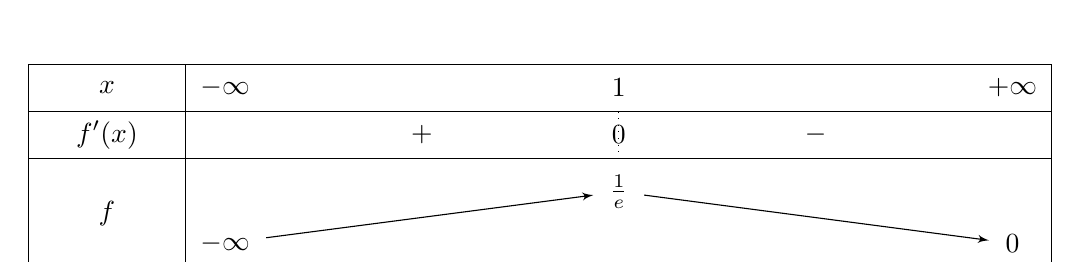
\begin{tikzpicture}
            \tkzTabInit[espcl=5]{$x$/0.6,$f'(x)$/0.6,$f$/1.4}{$-\infty$,$1$,$+\infty$}
            \tkzTabLine{,+,z,-,}
            \tkzTabVar{-/$-\infty$, +/$\frac{1}{e}$, -/$0$}
        \end{tikzpicture}
    \end{center}
    Alors, pour $x\in]-\infty,0]$, $|[x]|=1$, pour $x=1$, $|[x]|=1$ et sinon, $|[x]|=2$.\\
    \qed
\end{tcolorbox}
\addcontentsline{toc}{section}{\protect\numberline{}Exercice 16.1}

\section*{Exercice 16.2 [$\blacklozenge\blacklozenge\lozenge$]}
\begin{tcolorbox}[enhanced, width=7.6in, center, size=fbox, fontupper=\large, drop shadow southwest]
    On considère la relation $\mathcal{R}$ définie sur $\mathbb{N}^*$ par
    \begin{equation*}
        p ~ \mathcal{R} ~ q \iff \exists n \in \mathbb{N}^* ~ : ~ p^n = q.
    \end{equation*}
    Montrer que $\mathcal{R}$ est une relation d'ordre partiel sur $\mathbb{N}^*$.\\[0.15cm]
    Réfléxivité : Soit $p \in \mathbb{N}^*$. On a $p^1=p$, donc $p ~ \mathcal{R} ~ p$.\\[0.1cm]
    Antisymétrie : Soient $p,q\in\mathbb{N}^*$ tels que $\exists n \in \mathbb{N}^* ~ | ~ p^n = q$ et $\exists m \in \mathbb{N}^* ~ | ~ q^m = p$. Montrons que $p=q$.\\
    On a $p^n = q$ donc $p^{nm} = q^m = p$. De plus, $q^m = p$, donc $q^{nm} = p^n = q$.\\
    Ainsi, $p = p^{nm}$ et $q=q^{nm}$. Alors, soit $p = q = 1$, soit $n=m=1$ et alors $p=q$ dans tous les cas.\\[0.1cm]
    Transitivité : Soient $p,q,r \in \mathbb{N}^*$ tels que $\exists n \in \mathbb{N}^* ~ | ~ p^n = q$ et $\exists m \in \mathbb{N}^* ~ | ~ q^m = r$. Montrons que $p ~ \mathcal{R} ~ r$.\\
    On a que $p^{n} = q$ donc $p^{nm}=q^m=r$. Or $nm \in \mathbb{N}^*$, donc $p ~ \mathcal{R} ~ r$.\\[0.2cm]
    $\mathcal{R}$ est bien une relation d'ordre sur $\mathbb{N}^*$.\\
    Ce n'est pas un ordre total : il n'existe pas d'entier $n$ tel que $2^n=3$ ou $3^n=2$, par exemple.\\
    \qed
\end{tcolorbox}
\addcontentsline{toc}{section}{\protect\numberline{}Exercice 16.2}

\section*{Exercice 16.3 [$\blacklozenge\blacklozenge\lozenge$]}
\begin{tcolorbox}[enhanced, width=7.6in, center, size=fbox, fontupper=\large, drop shadow southwest]
    Soit $n\in\mathbb{N}^*$.\\
    Soient $x=(x_1,...,x_n)\in\mathbb{R}^n$ et $y=(y_1,...,y_n)\in\mathbb{R}^n$. On note $x \preceq y$ si
    \begin{equation*}
        \forall k \in \llbracket 1, n \rrbracket ~ : ~ \sum_{i=1}^kx_i \leq \sum_{i=1}^ky_i.
    \end{equation*}
    1. Montrer que $\preceq$ est une relation d'ordre sur $\mathbb{R}^n$.\\
    2. Si $n \geq 2$, montrer qu'il s'agit d'un ordre partiel.\\[0.2cm]
    1. Réfléxivité : Soit $x\in\mathbb{R}^n$. On a bien que $\forall k \in \llbracket 1,n \rrbracket ~\sum_{i=1}^kx_i \leq \sum_{i=1}^kx_i$.\\[0.1cm]
    Antisymétrie : Soient $x,y\in\mathbb{R}^n$. Supposons que $x \preceq y$ et $y \preceq x$. Montrons que $x=y$.\\
    On a que $\forall k \in \llbracket 1, n \rrbracket, ~ \sum_{i=1}^kx_i \leq \sum_{i=1}^ky_i ~ \wedge \sum_{i=1}^ky_i \leq \sum_{i=1}^kx_i$.\\
    Par antisymétrie de $\leq$, $\forall k \in \llbracket 1, n \rrbracket ~ \sum_{i=1}^kx_i = \sum_{i=1}^k y_i$.\\
    Par récurrence triviale sur $k$, on peut montrer que tous les éléments sont égaux 1 à 1.\\[0.15cm]
    Transitivité : Soient $x,y,z \in \mathbb{R}^n$ tels que $x \preceq y$ et $y \preceq z$. Montrons que $x \preceq z$.\\
    On a que $\forall k \in \llbracket 1, n \rrbracket, \sum_{i=1}^kx_i \leq \sum_{i=1}^ky_i\leq\sum_{i=1}^kz_i$. Par transitivité de $\leq$, $x \preceq z$.\\[0.2cm]
    2. Soient $x=(0,2)$ et $y=(1,0)$.\\
    On a $\sum_{i=1}^2x_i \geq \sum_{i=1}^2y_i$ et $\sum_{i=1}^1x_i \leq \sum_{i=1}^1y_i$ : $x$ et $y$ ne sont pas comparables, $\preceq$ est un ordre partiel.\\
    \qed
\end{tcolorbox}
\addcontentsline{toc}{section}{\protect\numberline{}Exercice 16.3}

\section*{Exercice 16.4 [$\blacklozenge\blacklozenge\lozenge$]}
\begin{tcolorbox}[enhanced, width=7.6in, center, size=fbox, fontupper=\large, drop shadow southwest]
    Sur $\mathbb{R}^*_+$, on définit une relation binaire en posant que deux réels strictement positifs sont en relation, ce qu'on note $x~\mathcal{R}~y$ si et seulement si
    \begin{equation*}
        \exists(p,q)\in(\mathbb{N}^*)^2 ~ px = qy
    \end{equation*}
    1. Démontrer que $\mathcal{R}$ est une relation d'équivalence.\\
    2. Démontrer que pour cette relation, deux classes d'équivalence sont nécessairement en bijection.\\[0.2cm]
    1. Réflexivité : Soit $x\in\mathbb{N}^*$. On a que $1\cdot x = 1\cdot x$ donc $x ~ \mathcal{R} ~ x$.\\
    Symétrie : Soient $x,y\in\mathbb{N}^*$ tels que $\exists(p,q)\in\mathbb{N}^* ~ px = qy$. On a $qy = px$ donc $y ~ \mathcal{R} ~ x$.\\
    Transitivité : Soient $x,y,z\in\mathbb{N}^*$ tels que $\exists(p,q)\in\mathbb{N}^*~px=qy$ et $\exists(p',q')\in\mathbb{N}^*~p'y=q'z$.\\
    On a $y=\frac{p}{q}x$ donc $p'\frac{p}{q}x=q'z$. Alors $pp'x=qq'z$ et $x~\mathcal{R}~z$.\\[0.15cm]
    2. Soient $[x]$ et $[y]$ deux classes d'équivalence de $\mathcal{R}$ avec $x,y\in\mathbb{R}^*_+$.\\
    On pose $f:\begin{cases}
        [x] \to [y]\\
        a\mapsto \frac{a}{x}y
    \end{cases}$.\\
    Pour $a\in[x]$, on a $f(a)\in[y]$ : $\exists (p,q)\in(\mathbb{N}^*)^2 ~ pa = qx$ Alors $a=\frac{q}{p}x$ et $f(a)=\frac{q}{p}\frac{x}{x}y \iff pf(a)=qy$.\\
    On a $f$ injective : Soient $a,a'\in[x]$ tels que $f(a)=f'(a)$ on a $\frac{y}{x}a=\frac{y}{x}a'$ donc $a=a'$.\\
    On a $f$ surjective : Soit $b\in[y]$ : $\exists(p,q)\in(\mathbb{N}^*)^2 ~ pb = qy$, alors $b=\frac{q}{p}y$.\\
    On pose $a\in[x] ~ | ~ pa=qx$, donc $a=\frac{q}{p}x$. On a $f(a)=\frac{q}{p}y=b$.\\
    Donc $f$ est bien une fonction bijective de $[x]$ vers $[y]$.
    \qed
\end{tcolorbox}
\addcontentsline{toc}{section}{\protect\numberline{}Exercice 16.4}

\section*{Exercice 16.5 [$\blacklozenge\blacklozenge\lozenge$]}
\begin{tcolorbox}[enhanced, width=7.6in, center, size=fbox, fontupper=\large, drop shadow southwest]
    Sur $\mathbb{R}$, on définit la relation $\mathcal{R}$ par
    \begin{equation*}
        x~\mathcal{R}~y \iff x^2 + 2y = y^2 + 2x.
    \end{equation*}
    1. Montrer que $\mathcal{R}$ est une relation d'équivalence sur $\mathcal{R}$.\\
    2. Déterminer la classe d'équivalence d'un réel a.\\[0.15cm]
    1. Réflexivité : On a bien que $x^2 + 2x = x^2 + 2x$.\\
    Symétrie : Soient $x,y\in\mathbb{R}$ tels que $x~\mathcal{R}~y$, par symétrie de l'égalité, on a $y~\mathcal{R}~x$.\\
    Transitivité : Soient $x,y,z\in\mathbb{R}$ tels que $x~\mathcal{R}~y$ et $y~\mathcal{R}~z$. Par transitivité de l'égalité, $x~\mathcal{R}~z$.\\[0.15cm]
    2. Soit $x\in\mathbb{R}$. On a :
    \begin{align*}
        &x^2 + 2a = a^2 + 2x\\
        \iff&x^2 - a^2 = 2(x-a)\\
        \iff&(x-a)(x+a)=2(x-a)\\
        \iff&(x-a)(x+a-2)=0
    \end{align*}
    Ainsi, soit $x=a$, soit $x=2-a$.\\
    La classe d'équivalence de $a$ est alors : $[a]=\{2-a,a\}$.\\
    \qed
\end{tcolorbox}
\addcontentsline{toc}{section}{\protect\numberline{}Exercice 16.5}

\section*{Exercice 16.6 [$\blacklozenge\blacklozenge\lozenge$]}
\begin{tcolorbox}[enhanced, width=7.6in, center, size=fbox, fontupper=\large, drop shadow southwest]
    Soit $\mathcal{R}$ une relation sur un ensemble $E$.\\
    Pour $x,y\in E$, on note $x \sim y$ s'il existe $n\in\mathbb{N}^*$ et $x_0,...x_n$ tels que
    \begin{equation*}
        x_0 = x, ~ x_0 ~ \mathcal{R} ~ xx_1, ~ x_1 ~ \mathcal{R} ~ x_2, ~ ..., ~ x_{n-1} ~ \mathcal{R} ~ x_n, ~ x_n = y.
    \end{equation*}
    1. Montrer que $\sim$ est une relation transitive sur $E$.\\
    2. On suppose $\mathcal{R}$ transitive et symétrique. Montrer que $\sim$ est une relation d'équivalence sur $E$.
\end{tcolorbox}
\addcontentsline{toc}{section}{\protect\numberline{}Exercice 16.6}

\end{document}
 
